\documentclass[12pt]{extarticle}
\usepackage{tempora}
\usepackage[T1, T2A]{fontenc}
\usepackage[utf8]{inputenc}
\usepackage[english, ukrainian]{babel}
\usepackage{geometry}
\usepackage{graphicx}
\usepackage{multirow}
\usepackage{multicol}
\usepackage{float}
\graphicspath{{/home/artem/Pictures}}
\geometry
{
    a4paper,
    left=30mm,
    top=15mm,
    right=20mm,
    bottom=15mm,
}

\begin{document}
\begin{titlepage}
    \begin{center}
        \textbf{\normalsize{\MakeUppercase{
            Міністерство Освіти і науки України
            Національний університет "Львівська політехніка"
        }}}

        \begin{flushright}
        \textbf{ІКНІ}\\
        Кафедра \textbf{ПЗ}
        \end{flushright}
        \vspace{15mm}

        \includegraphics[width=0.4\textwidth]{lpnu_logo.png}

        \vspace*{\fill}

        \textbf{\normalsize{\MakeUppercase{Звіт}}}
            
        До лабораторної роботи №5

        \textbf{на тему:} “Багатопоточність в операційній сисемі WINDOWS. Створення,
        керування та синхронізація потоків.”

        \textbf{з дисципліни:} “Операційні системи”
            
        \vspace*{\fill}

        \begin{flushright}

            \textbf{Лектор:}\\
            старший викладач кафедри ПЗ\\
            Грицай О.Д.\\
            \vspace{12pt}

            \textbf{Виконав:}\\
            студент групи ПЗ-24\\
            Губик А. С.\\
            \vspace{12pt}

            \textbf{Прийняв:}\\
            доцент кафедри ПЗ\\
            Горечко О. М.\\
        \vspace{12pt}
        \end{flushright}

        Львів -- 2023
            
            
    \end{center}
\end{titlepage}

\textbf{Тема роботи:}Багатопоточність в операційній сисемі WINDOWS. Створення,
керування та синхронізація потоків.
\vspace{12pt}

\textbf{Мета роботи:}Ознайомитися з багатопоточністю в ОС Windows. Навчитись
реалізовувати розпаралелення алгоритмів за допомогою багатопоточності в ОС
Windows з використанням функцій WinAPI. Навчитись використовувати різні
механізми синхронізації потоків.

\subsection*{Теоретичні відомості}
Розглядаючи поняття процесу, визначають ще одну абстракцію для
запущеного процесу: потік. У класичному уявленні існує єдина точка виконання
в рамках програми (тобто єдиний потік контролю, на якому збираються та
виконуються інструкції), багатопотокова програма має більш ніж одну точку
виконання (тобто кілька потоків контролю, кожен з яких який отримується та
виконується).
Кожен потік дуже схожий на окремий процес, за винятком однієї відмінності:
вони мають спільний адресний простір і, отже, мають доступ до одних і тих же
даних. Таким чином, стан одного потоку дуже подібний до стану процесу. Він
має лічильник програм (PC), який відстежує, звідки програма отримує інструкції.
Кожен потік має свій власний приватний набір реєстрів, який він використовує
для обчислень; таким чином, якщо на одному процесорі працюють два потоки,
при переході від запуску одного (T1) до запуску іншого (T2) має відбутися
перемикання контексту. Контекстний перемикач між потоками дуже подібний до
перемикання контекстів між процесами, оскільки перед запуском Т2 необхідно
зберегти регістр стану Т1 і відновити стан реєстру Т2. За допомогою процесів ми
зберегли стан до блоку управління процесами (PCB); тепер нам знадобиться
один або кілька блоків управління потоками (TCB) для збереження стану
кожного потоку процесу. Однак є одна істотна відмінність у перемиканні
контексту, який ми виконуємо між потоками порівняно з процесами: адресний
простір залишається незмінним (тобто немає необхідності змінювати, яку
таблицю сторінок ми використовуємо).
Ще одна істотна відмінність між потоками та процесами стосується стека. У
простій моделі адресного простору класичного процесу (однопотокового) є
єдиний стек, який зазвичай знаходиться внизу адресного простору. Однак у
багатопотоковому процесі кожен потік працює окремо і, звичайно, може
залучати різні підпрограми для виконання будь -якої роботи. Замість одного
стека в адресному просторі буде по одному на кожен потік.
\subsection*{Індивідуальне завдання}

Бінарний пошук максимального елементу масиву (кількість елементів
>10000, елементи рандомні). Вивести значення та індекс. Синхронізація: 2, 8
\begin{enumerate}
    
\item Мютекс
\item Семафор
\item Інтерлок-функції
\item Критична секція
\item Події
\item Функції очікування
\item Алгоритм активного очікування
\item Алгоритм монітору
\item Таймери очікування
\end{enumerate}
\subsection*{Хід роботи}


\paragraph{I.} Розпаралелення бінарного пошуку на 2, 4, 8, 16 потоків
\begin{figure}[H]
    \centering
    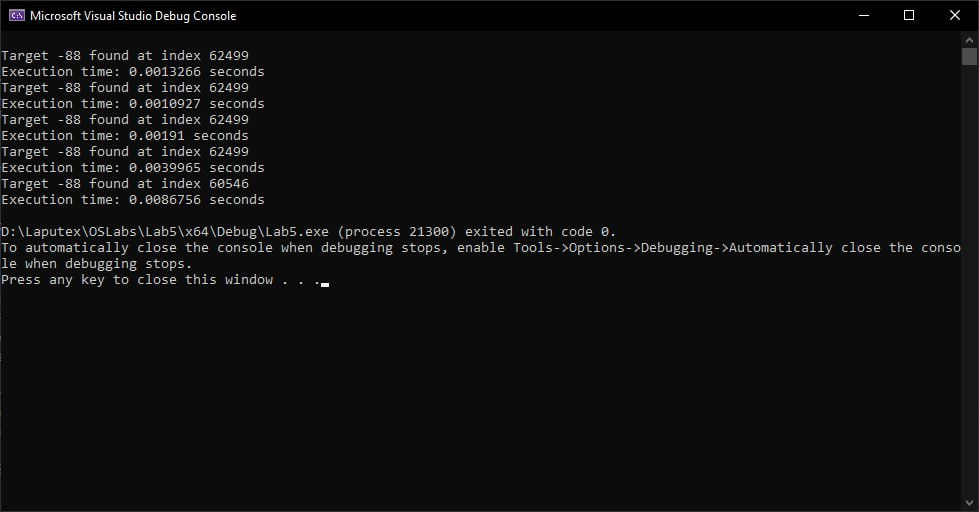
\includegraphics[width=0.90\textwidth]{no_sync.jpg}
    \caption{Без синхронізації}
\end{figure}
\begin{figure}[H]
    \centering
    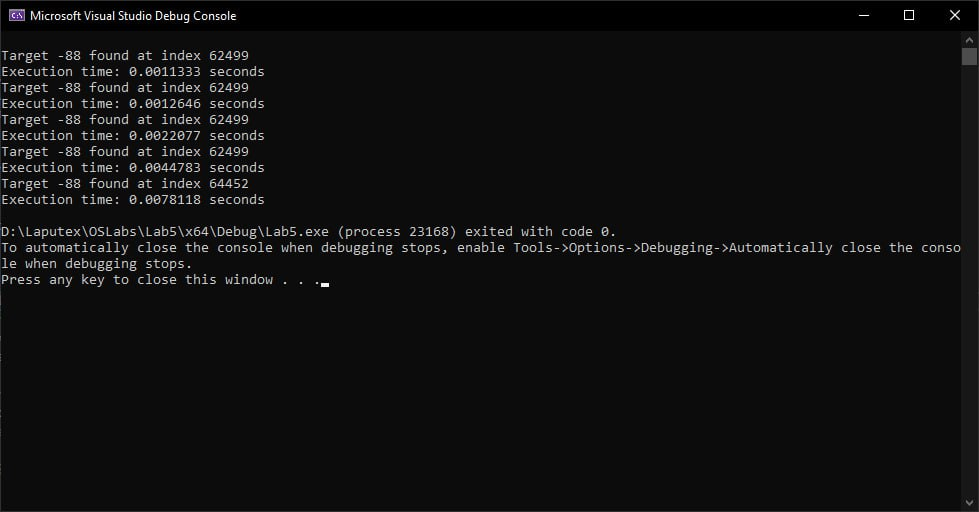
\includegraphics[width=0.90\textwidth]{semaphore.jpg}
    \caption{З використанням семафори}
\end{figure}
\begin{figure}[H]
    \centering
    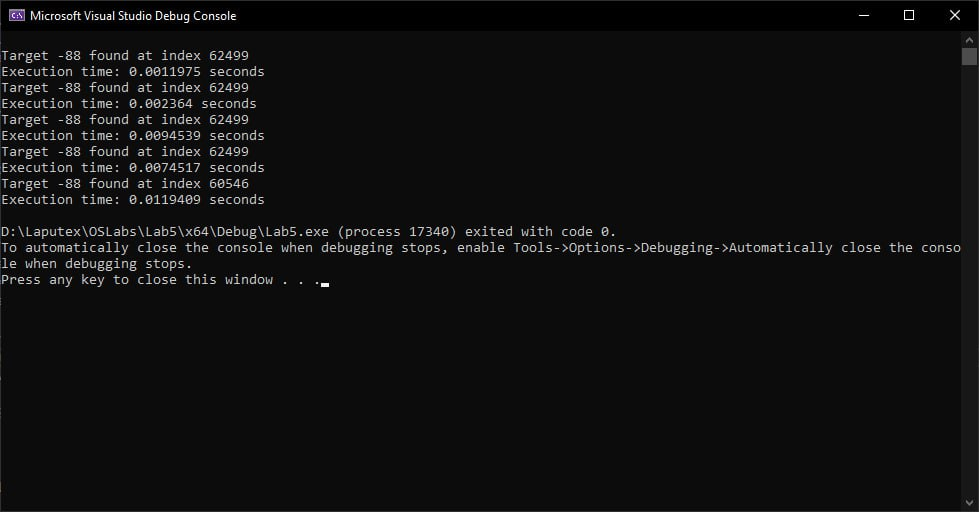
\includegraphics[width=0.90\textwidth]{monitor.jpg}
    \caption{}
\end{figure}

Як бачимо синхронізація сповільнює роботу і не впливає на правильність виконання бінарного пошуку.


\break

\paragraph{II.} Зупинка потоків
\begin{figure}[H]
    \centering
    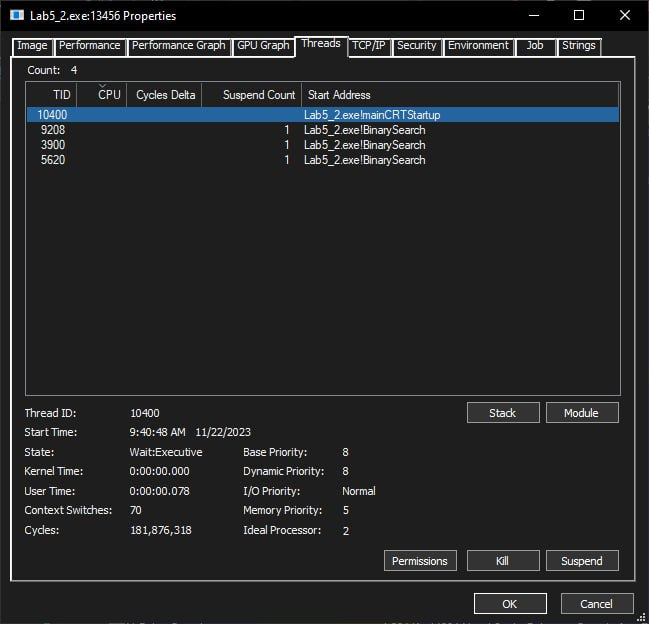
\includegraphics[width=0.90\textwidth]{threads.jpg}
    \caption{Process explorer properties}
\end{figure}
\textbf{Висновок:}
Ефективність синхронізації залежить від поставленої перед нами задачі. У
випадку з бінарним пошуком воно не потрібне і сповільнює роботу.
 \end{document}
